%%%%%%%%%%%%%%%%%%%%%%%%%%%%%%%%%%%%%%%%%%%%%%%%%%%%%%%%%%%%%%%%%%%%%%%%%%%%%%
\newpage
\section {Reconstruction }

Distributions of the reconstructed track momentum and T0 for all reconstructed positive
tracks from $\pi^+ \to e^+ \nu $ decays in the ST are shown in Figure~\ref{fig:all_tracks_p_t0}.
The distributions corresponding to different degrader thicknesses are overlaid.
One can see that the probability per POT to have a reconstructed positron track reaches its maximum
for degrader thicknesses of about 2-3 mm Ti, and it starts falling down as the degrader thickness
increases.

Compared to ``no degrader'', a 2-3mm thick Ti degrader increases the acceptance by a factor
close to x3.

\begin{figure}[H]
  % \centering
  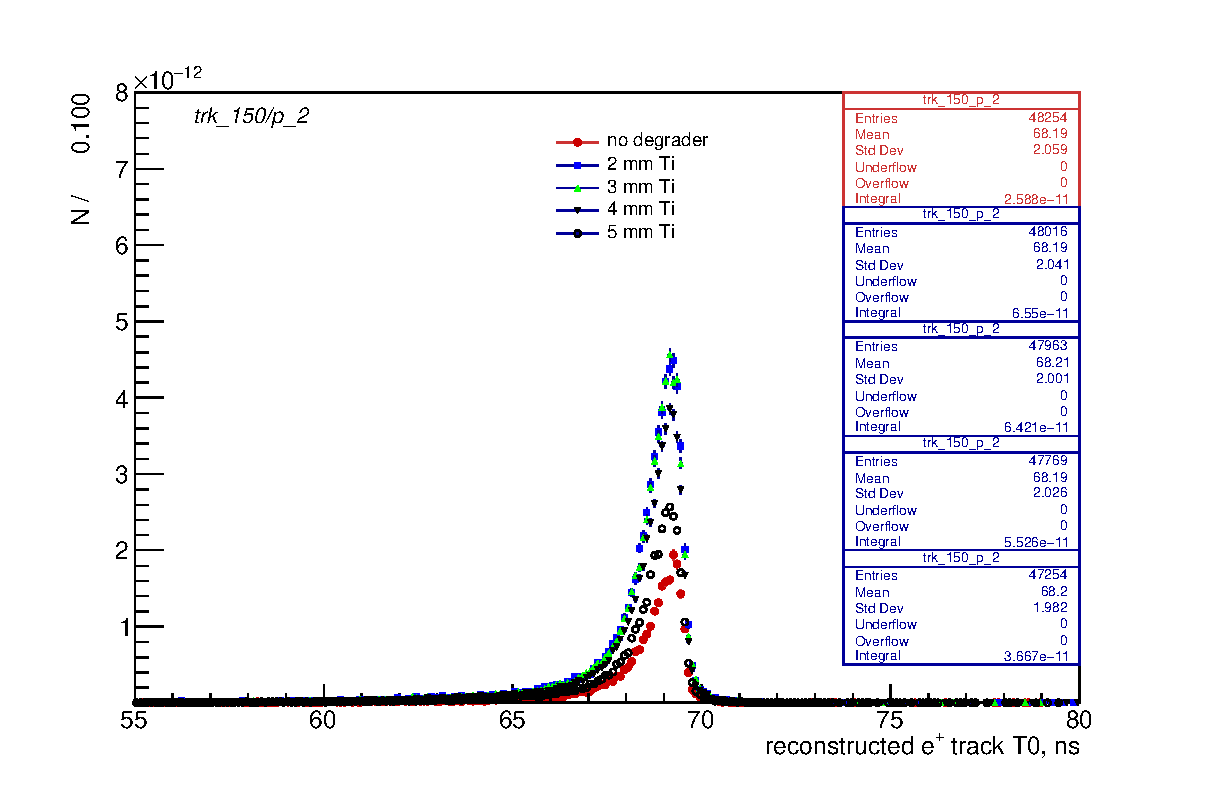
\includegraphics[width = 0.55\linewidth]{pdf/figure_00001}
  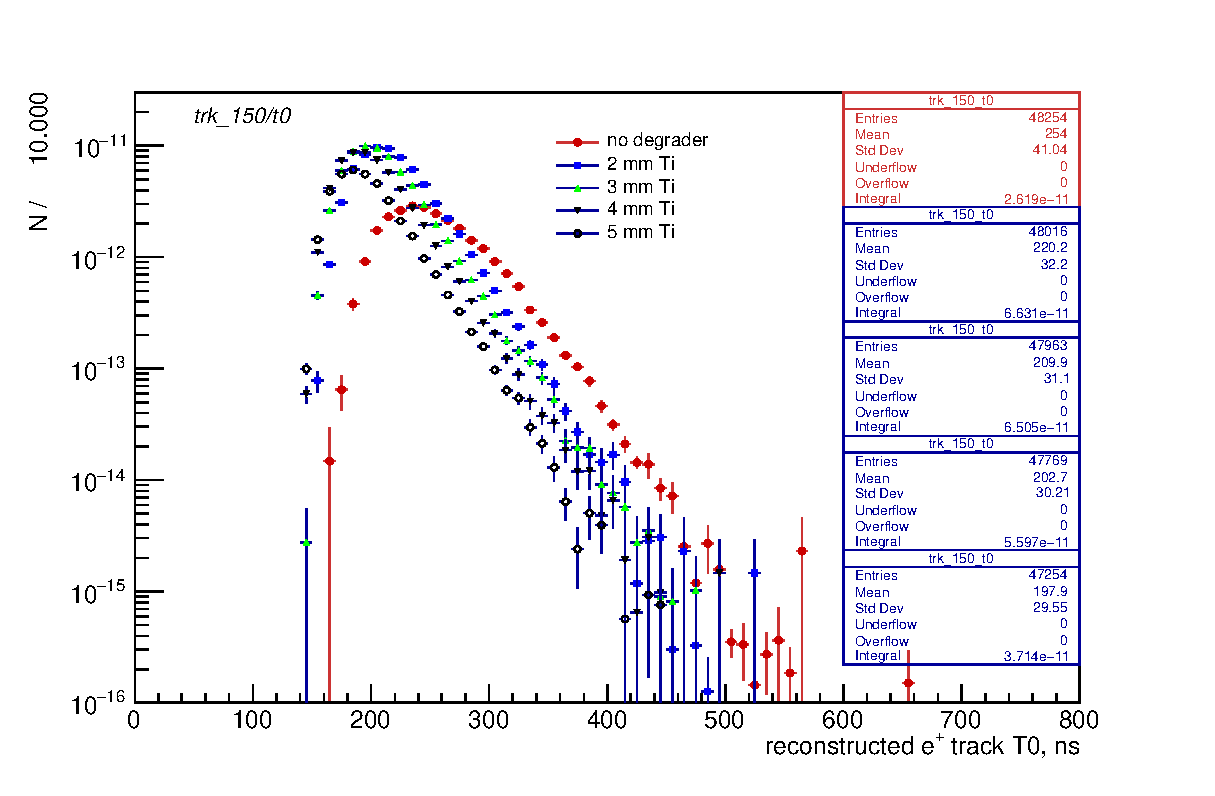
\includegraphics[width = 0.55\linewidth]{pdf/figure_00002}
  \caption{
    \label{fig:all_tracks_p_t0}
    Distributions of the reconstructed ST $\pi^+ \to e^+ \nu$ track momentum and time
    for different degrader thicknesses
  }
\end{figure}

%%%%%%%%%%%%%%%%%%%%%%%%%%%%%%%%%%%%%%%%%%%%%%%%%%%%%%%%%%%%%%%%%%%%%%%%%%%%%%
\subsection{Track selection cuts}

Give a table of initial track selection cuts - close to ``Set C''...

\begin{figure}[H]
  % \centering
  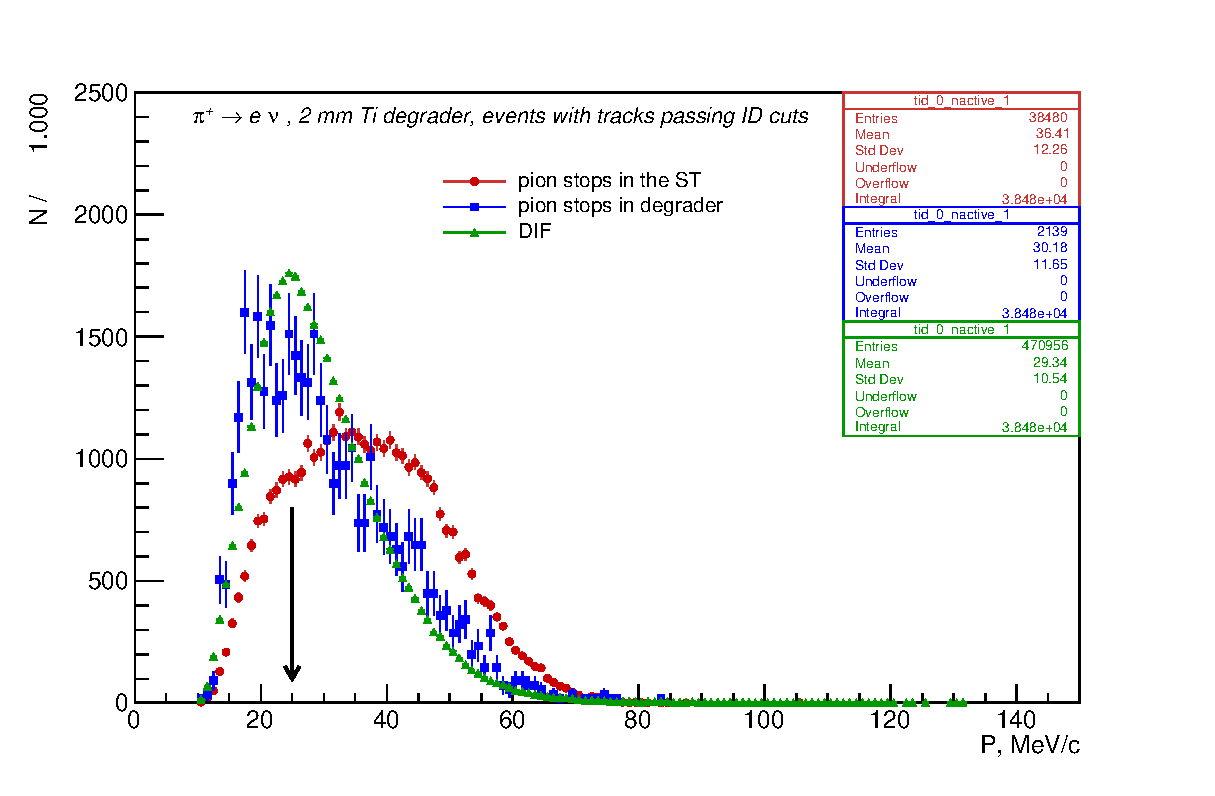
\includegraphics[width=0.55\linewidth]{pdf/figure_00274}  % tid_0/nactive_1
  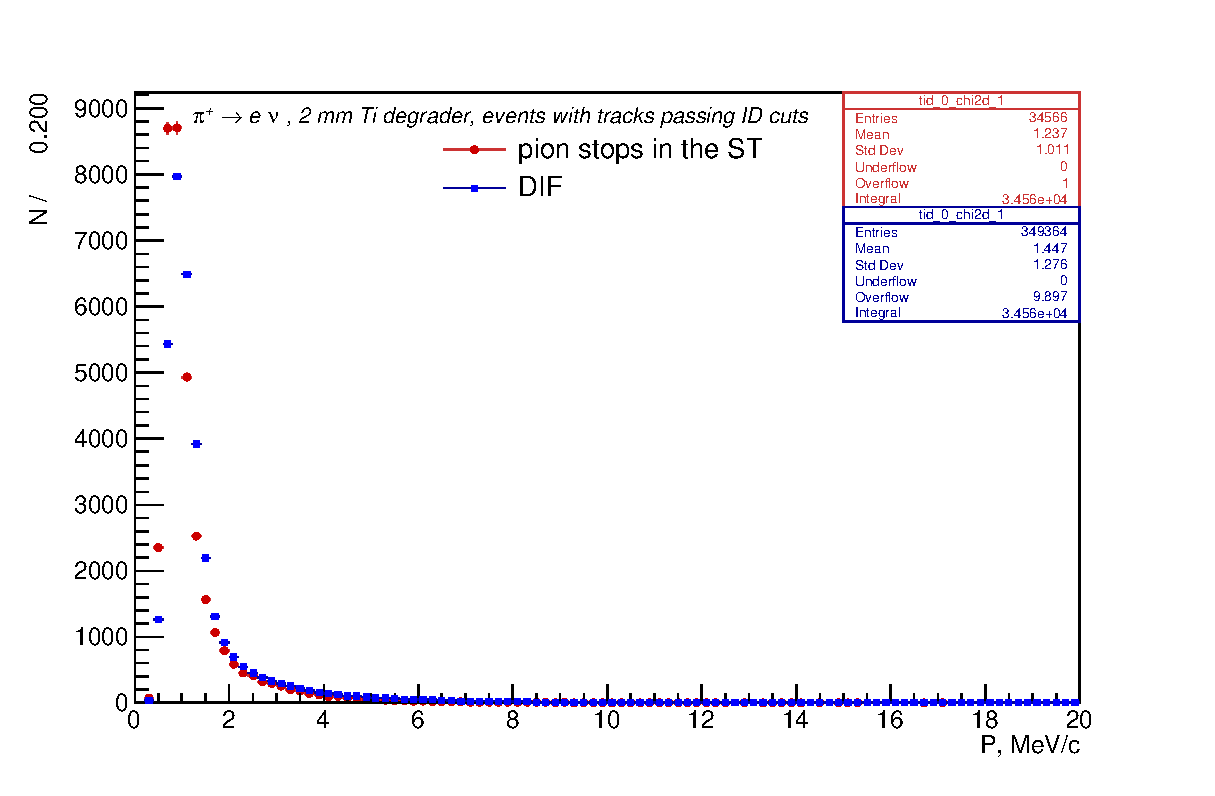
\includegraphics[width=0.55\linewidth]{pdf/figure_00275}  % tid_0/chi2d_1
  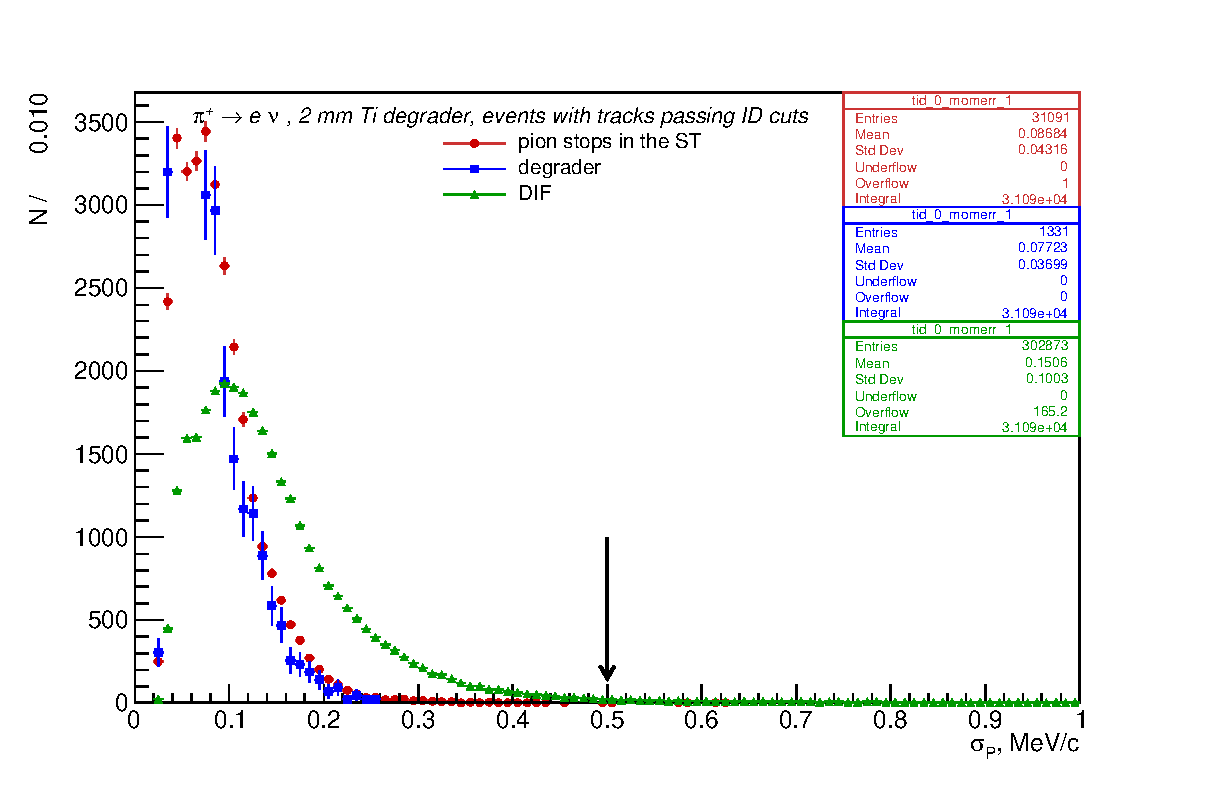
\includegraphics[width=0.55\linewidth]{pdf/figure_00276}  % tid_0/momerr_1
  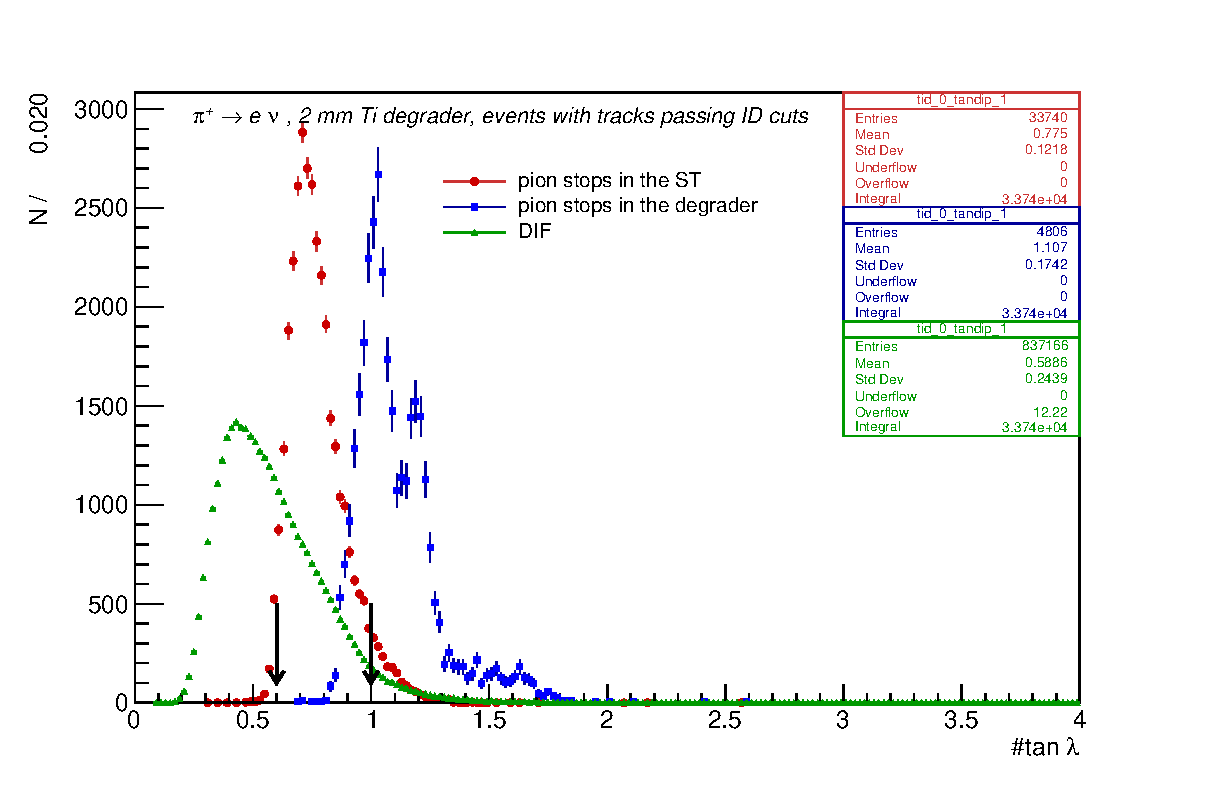
\includegraphics[width=0.55\linewidth]{pdf/figure_00273}  % tid_0/tandip_1
  \caption{
    \label{fig:tid_variables}
    Distributions of the track ID variables 
  }
\end{figure}

Based on the distributions in the track ID variables presented in Figure~\ref{fig:tid_variables},
we adopt the track ID cuts shown in the Table~\ref{table:track_id_cuts}
\begin{table}[H]
  \centering
  \begin{tabularx} {0.5\textwidth}{|X|c|}  %
    \hline
    variable                &   cut                        \\
    \hline                         
    N hits used by the fit &   $N_{active}>= 25$            \\
    \hline                         
    chi2/DOF             &   $\chi2/DOF < 3$            \\
    \hline                         
    track dip angle     &   $0.6 < \tan \lambda < 1.0$ \\
    \hline                         
    track momentum error    &   $\sigma_P < 0.5$ MeV/c     \\
    \hline
  \end{tabularx}
  \caption{
    \label{table:track_id_cuts}
    Track ID cuts
  }
\end{table}

It is worth noticing that the cut on the track dip angle significantly reduces
the contribution of positrons coming from $\pi^+ \to e^+ \nu$ decays in the degrader.

%%%%%%%%%%%%%%%%%%%%%%%%%%%%%%%%%%%%%%%%%%%%%%%%%%%%%%%%%%%%%%%%%%%%%%%%%%%%%%
\subsection{Signal reconstruction efficiency}

%% to see the number of entries and the weight, plot murat_pipenu_ana:trk_150/p_2

\begin{table}[H]
\begin{tabularx}{1.0\textwidth} {|X|c|c|c|c|c|c|}  %
% \begin{tabular}{1.0\textwidth} {|l|l|}  %
  \hline
 degrader thickness &   Dataset  &N(simulated) & N(reco tracks) & sum W   & N(reco tracks) & sum W        \\
 (mm)               &            &             &     ST         &   ST    &    degrader    &  degrader    \\
  \hline                                                                          
  no degrader       &   bpip0b0  &  100000     &    48254       &  17.03  &     0          &              \\
  \hline                                                                          
     2              &   bpip2b0  &  100000     &    48016       &   159    &   10198       &   13.18      \\
  \hline                                                                         
     3              &   bpip3b0  &  100000     &    47963       &   262.6  &    7779       &   20.97       \\
  \hline                                                                         
     4              &   bpip4b0  &  100000     &    47769       &   359.1  &    5910       &   25.76       \\
  \hline                                                                          
     5              &   bpip5b0  &  100000     &    47254        &  428.3  &    4452       &   27.12       \\
  \hline
\end{tabularx}
  \caption{
    % \label{fig:deg_vs_no_degrader_time}
    Number of the events with reconstructed tracks for different pion datasets
  }
\end{table}

%%%%%%%%%%%%%%%%%%%%%%%%%%%%%%%%%%%%%%%%%%%%%%%%%%%%%%%%%%%%%%%%%%%%%%%%%%%%%%
\newpage
\subsection{Decays of pions stopped in the degrader}

Reconstructed momentum distributions for positrons from $\pi^+ \to e^+ \nu$ decays
in the ST and degrader are shown in Figure~\ref{fig:stt_vs_deg_momentum_good_tracks}

% \begin{figure}[H]
%   % \centering
%   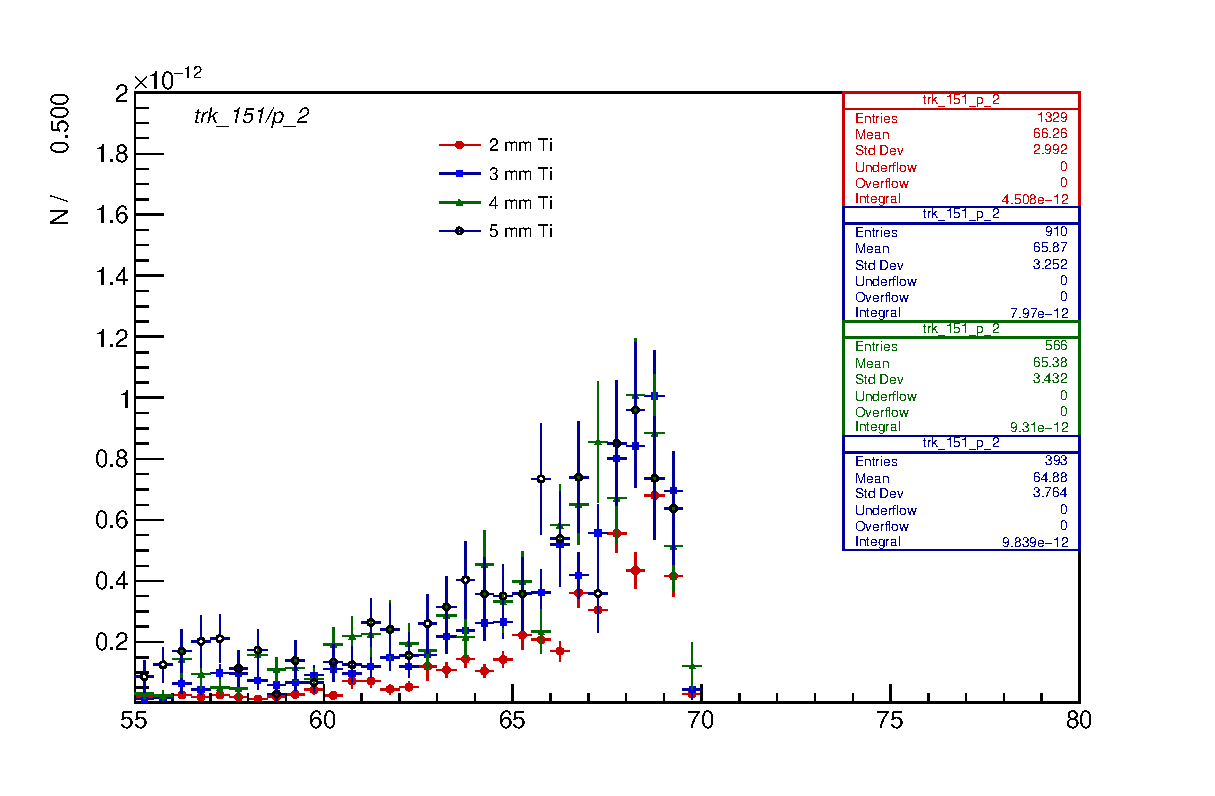
\includegraphics[width=0.55\linewidth]{pdf/figure_00041}
%   \caption{
%     \label{fig:degrader_good_track_mom}
%   }
% \end{figure}

% \begin{figure}[H]
%   % \centering
%   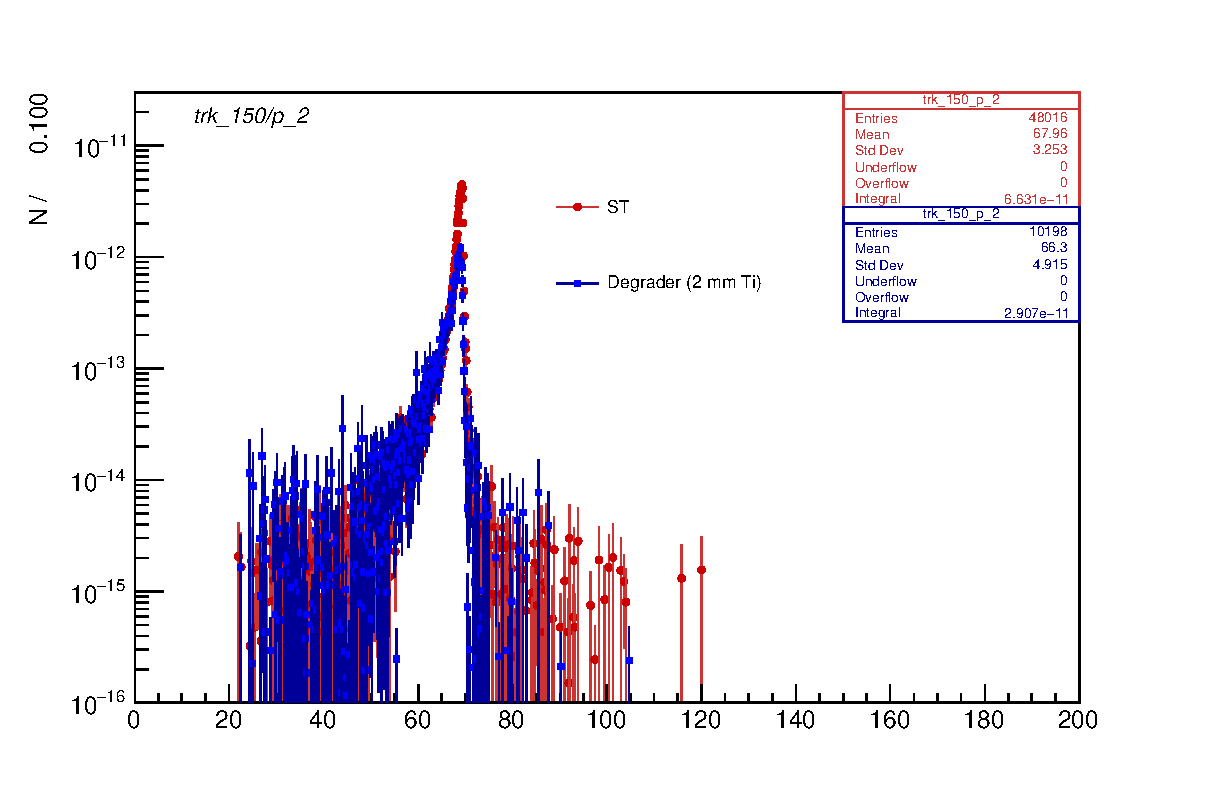
\includegraphics[width=0.55\linewidth]{pdf/figure_00201}
%   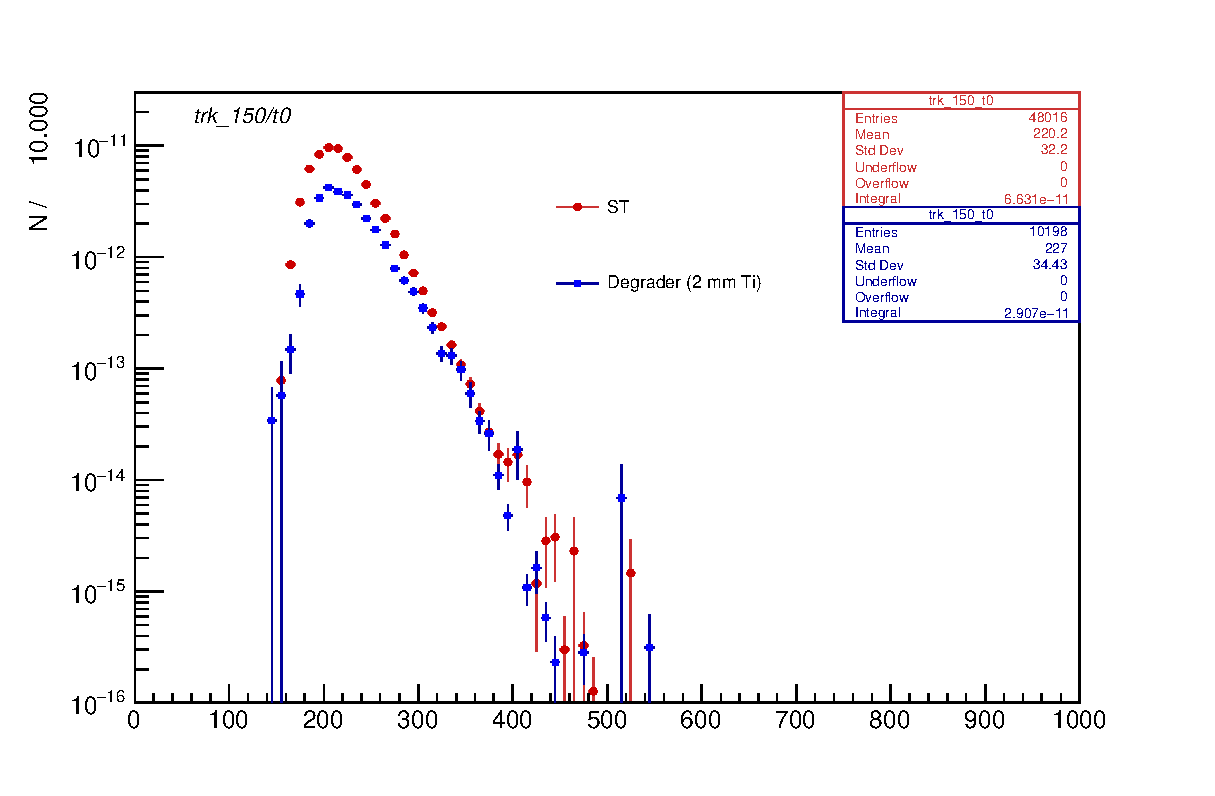
\includegraphics[width=0.55\linewidth]{pdf/figure_00202}
%   \caption{
%     % \label{fig:deg_vs_no_degrader_time}
%   }
% \end{figure}

% \begin{figure}[H]
%   % \centering
%   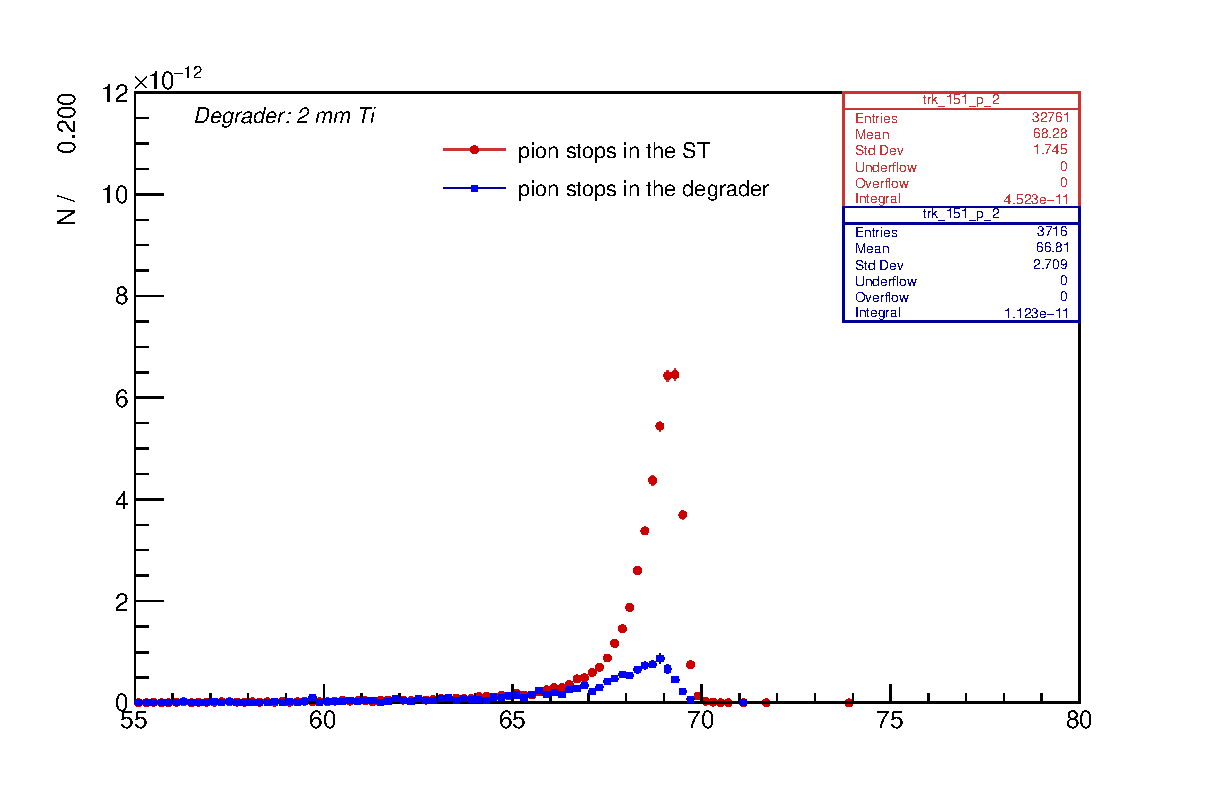
\includegraphics[width=0.55\linewidth]{pdf/figure_00211}
%   \caption{
%     % \label{fig:deg_vs_no_degrader_time}
%   }
% \end{figure}

% \begin{figure}[H]
%   % \centering
%   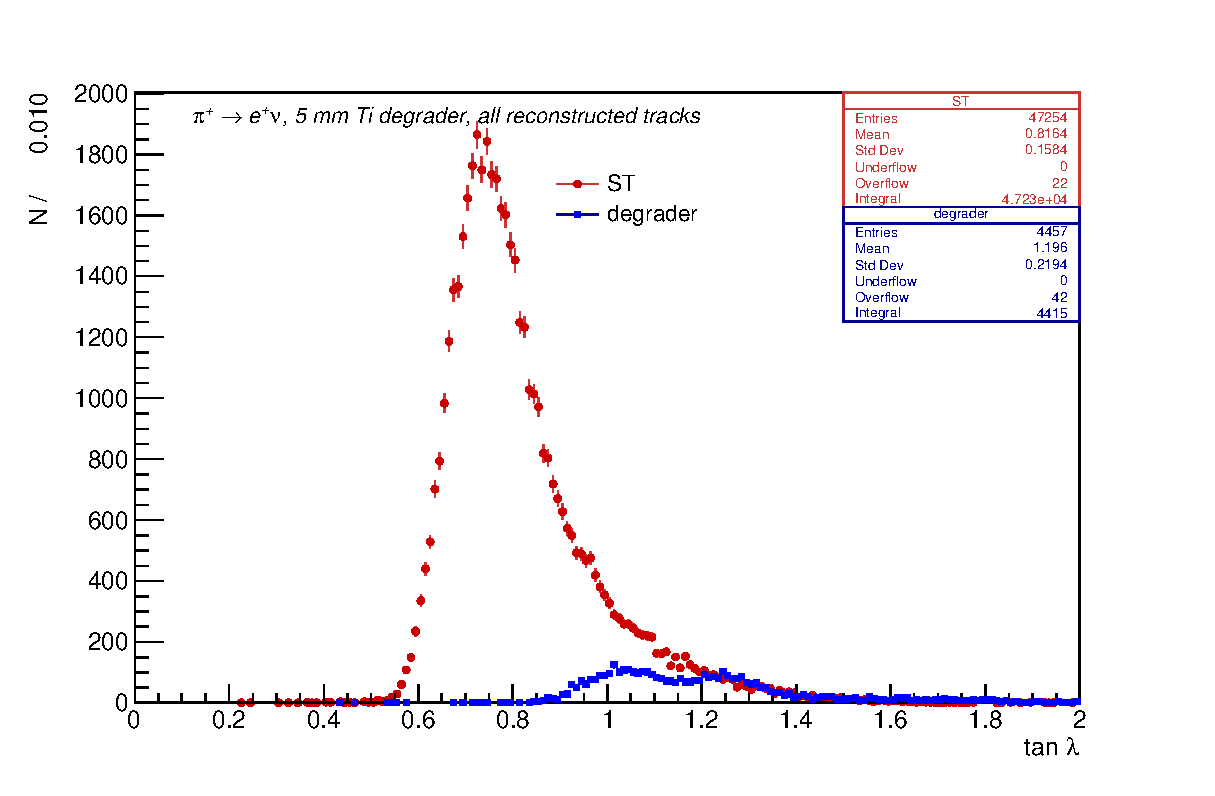
\includegraphics[width=0.55\linewidth]{pdf/figure_00503}
%   \caption{
%     % \label{fig:deg_vs_no_degrader_time}
%     track ID variables, 5 mm Ti degrader, all reconstructed tracks
%   }
% \end{figure}

\begin{figure}[H]
  % \centering
  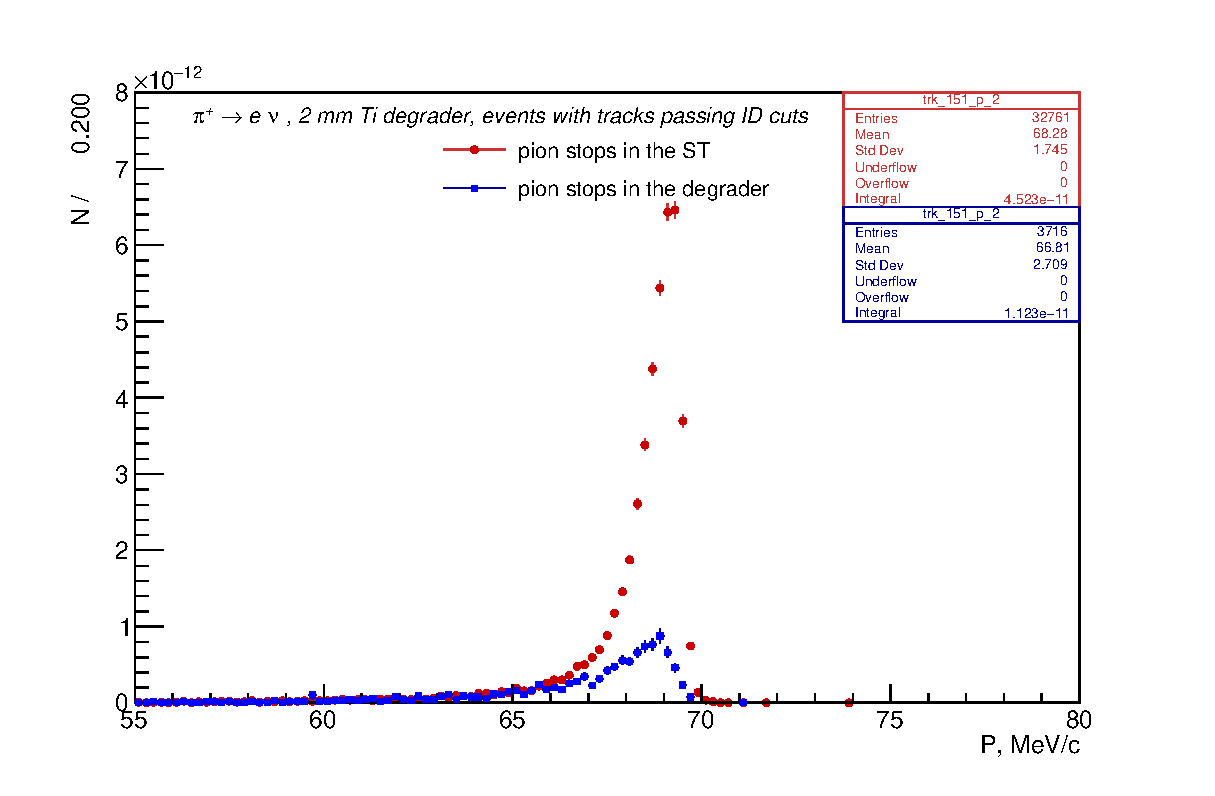
\includegraphics[width=0.55\linewidth]{pdf/figure_00261}
  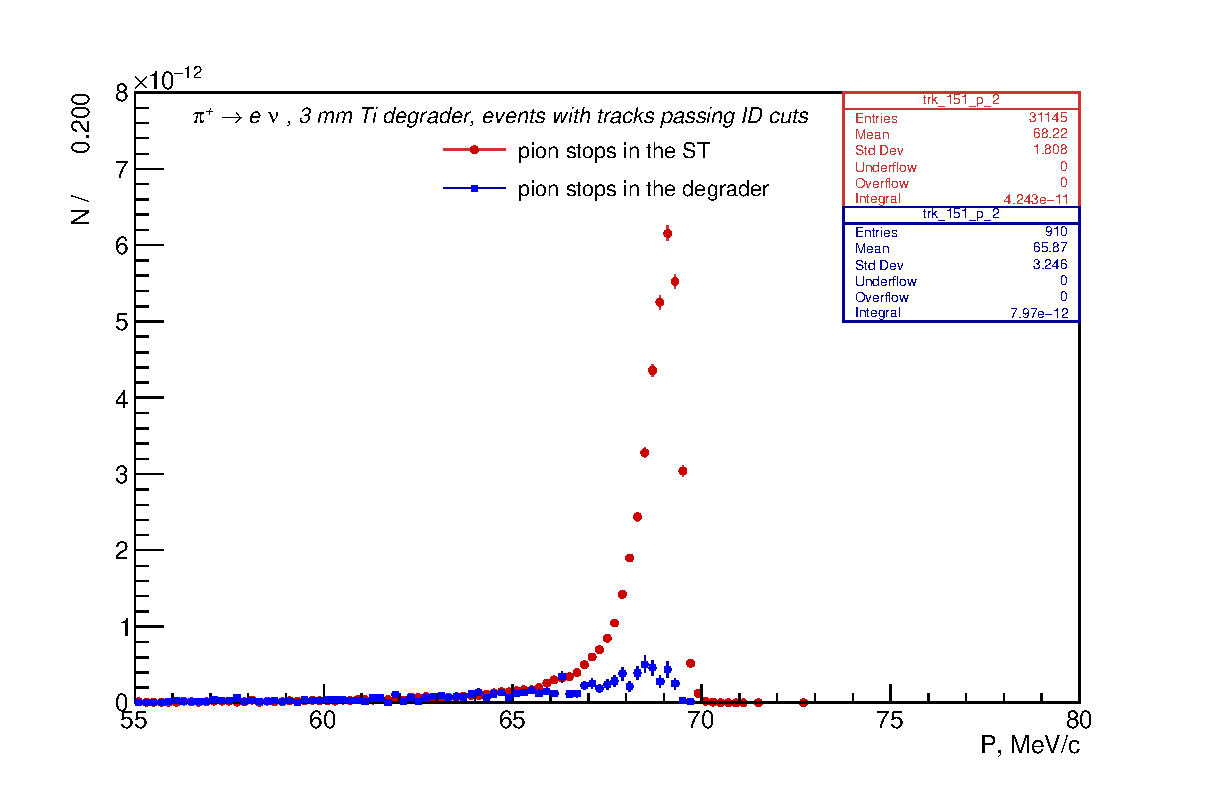
\includegraphics[width=0.55\linewidth]{pdf/figure_00361}
  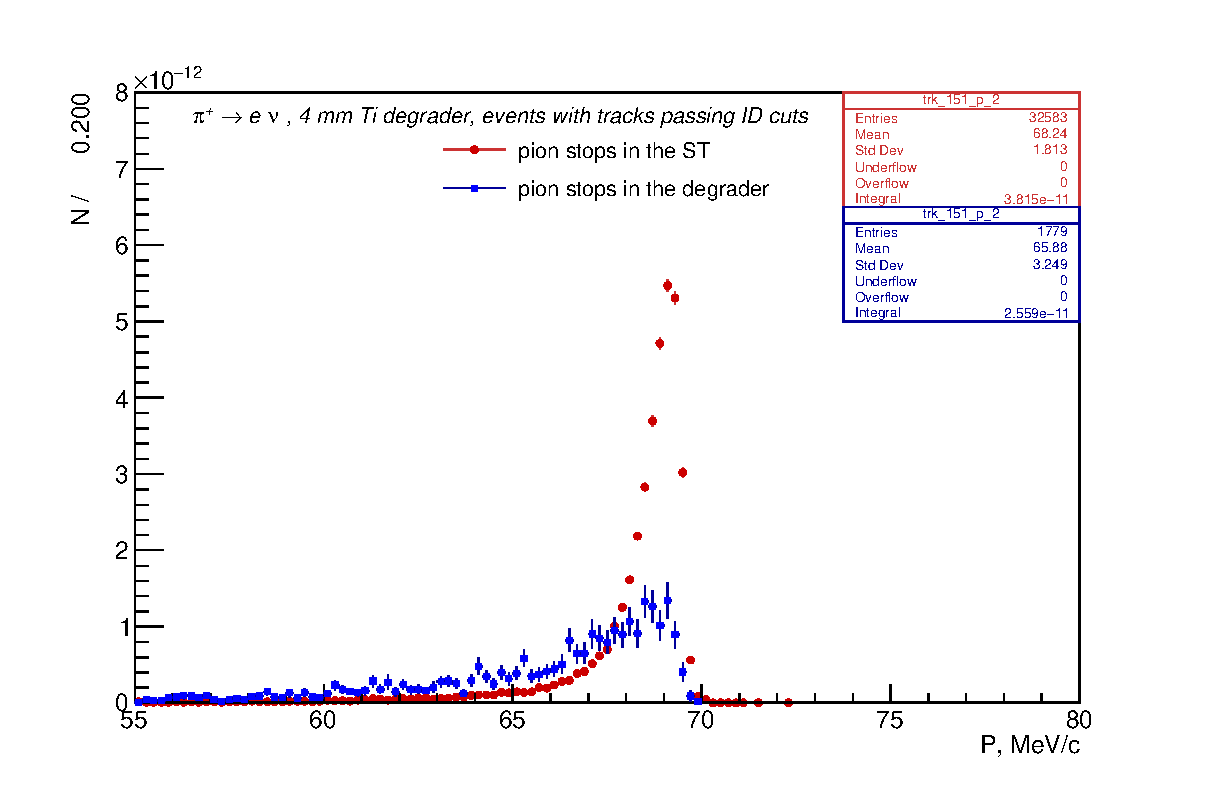
\includegraphics[width=0.55\linewidth]{pdf/figure_00461}
  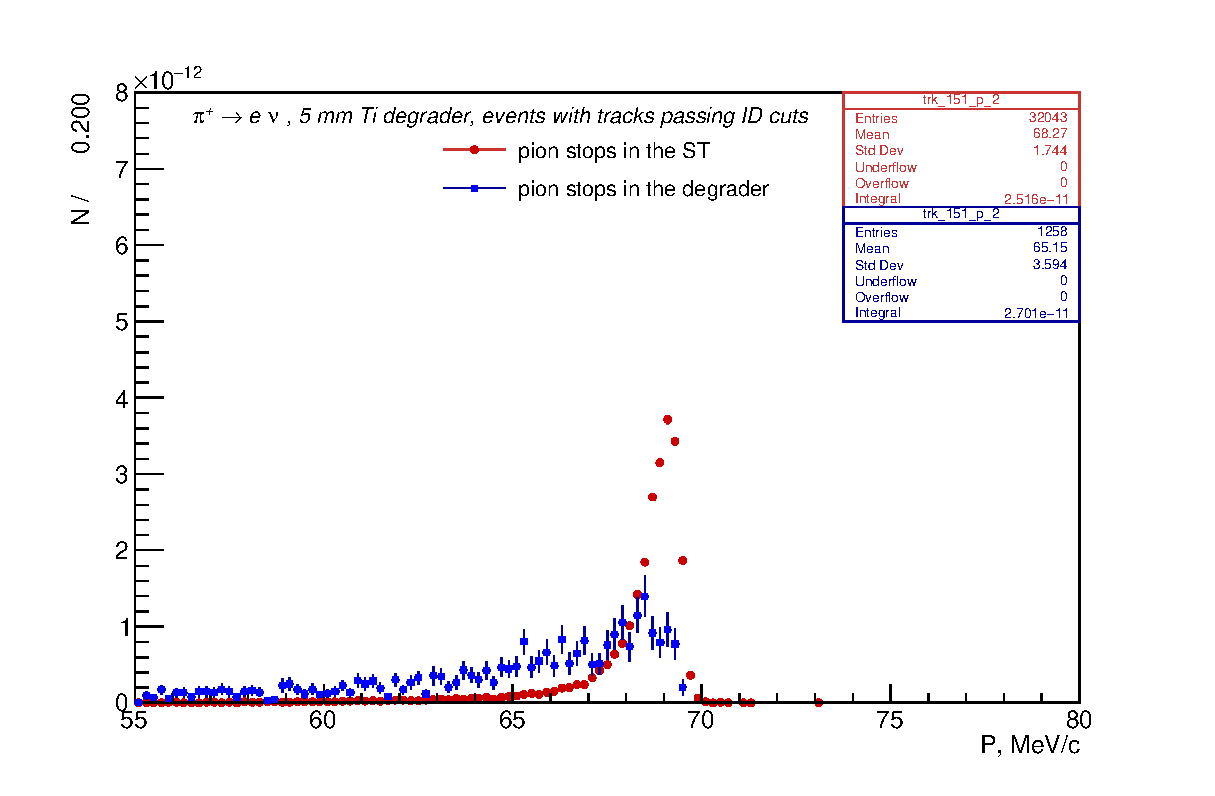
\includegraphics[width=0.55\linewidth]{pdf/figure_00561}
  \caption{
    \label{fig:stt_vs_deg_momentum_good_tracks}
    reconstructed e+ yield/POT for different degrader thicknesses, STT vs DEG
  }
\end{figure}

For the signal window $67.5 < P < 70$ MeV/c, the relative contribution of pion
decays in degrader is in the range of 10-15\%.

Timing distributions are shown if Figure~\ref{figure:stt_vs_deg_t0_good_tracks}.
As, on average, slower pions stop in the degrader, the degrader timing distributions
fall a little bit slower.
Therefore, at large T0 the contribution of the degrader stops increases.


\begin{figure}[H]
  % \centering
  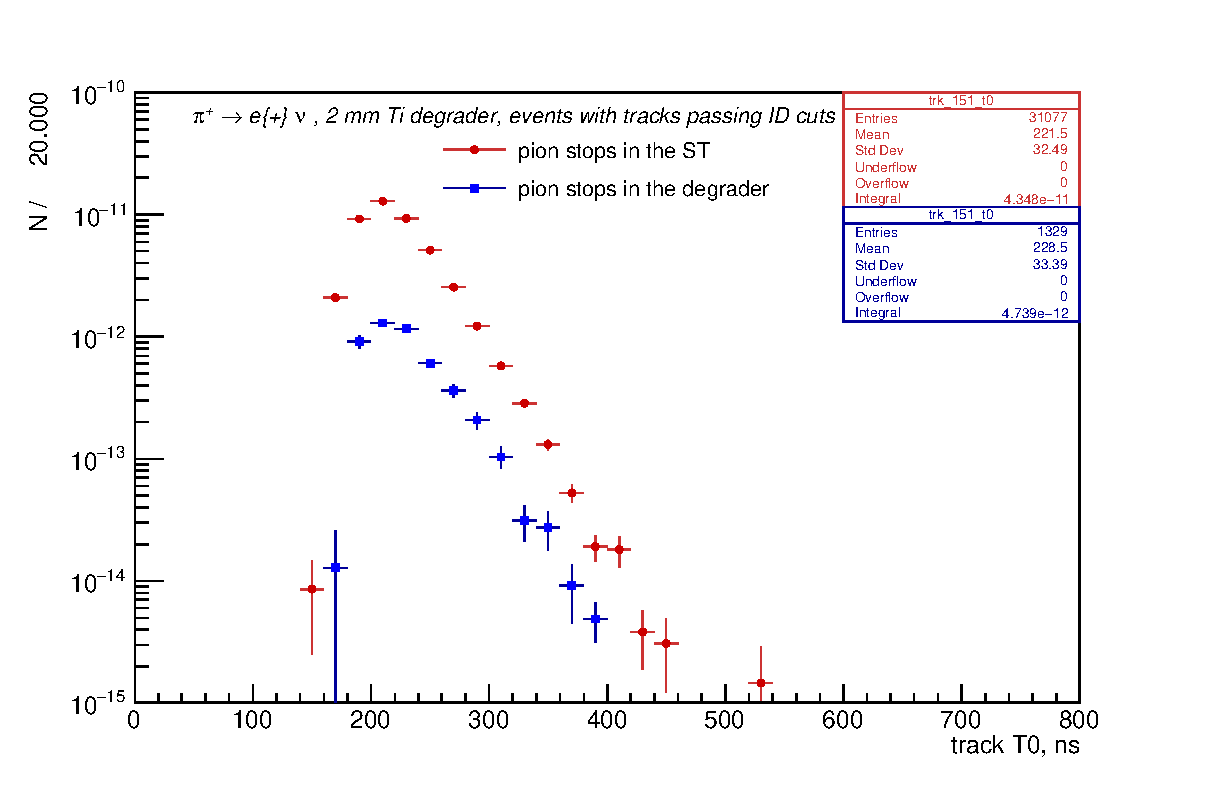
\includegraphics[width=0.55\linewidth]{pdf/figure_00262}
  \includegraphics[width=0.55\linewidth]{pdf/figure_00362}
  \includegraphics[width=0.55\linewidth]{pdf/figure_00462}
  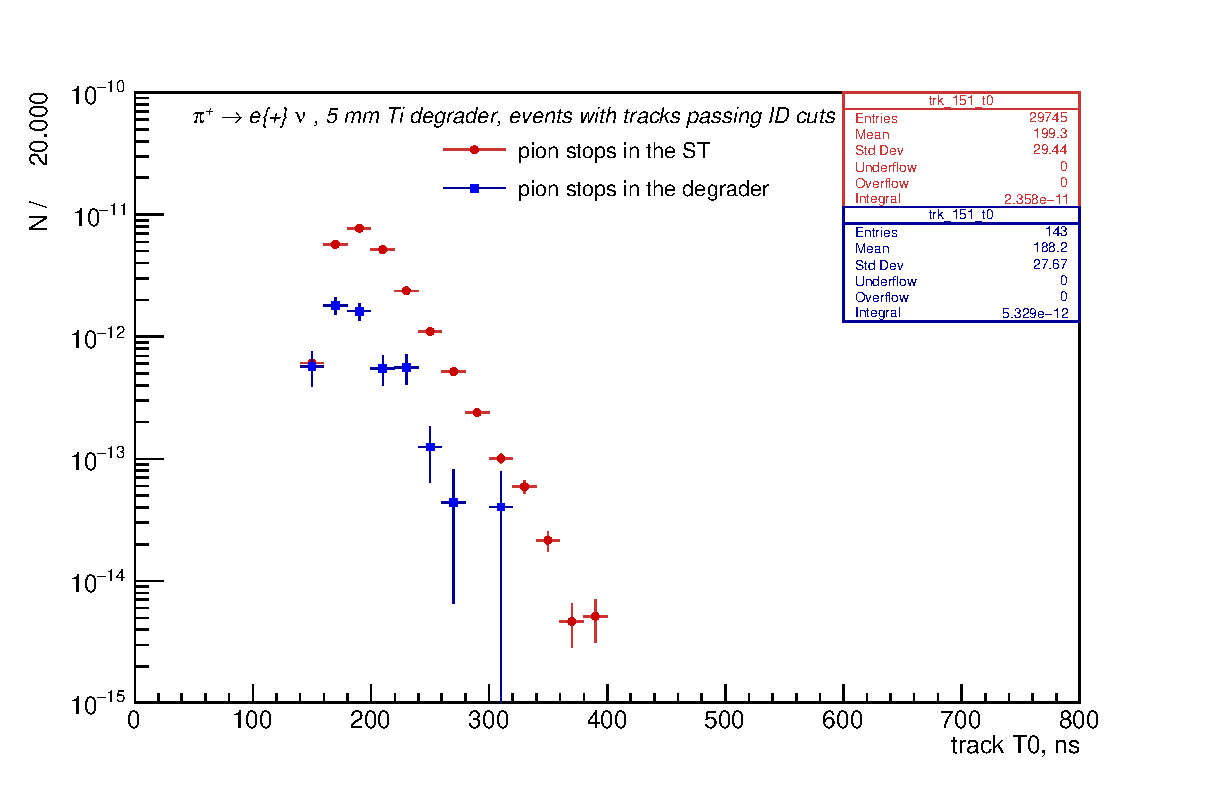
\includegraphics[width=0.55\linewidth]{pdf/figure_00562}
  \caption{
    \label{figure:stt_vs_deg_t0}
    reconstructed e+ yield/POT for different degrader thicknesses, STT vs DEG
  }
\end{figure}

%%%%%%%%%%%%%%%%%%%%%%%%%%%%%%%%%%%%%%%%%%%%%%%%%%%%%%%%%%%%%%%%%%%%%%%%%%%%%%
\section{Signal selection efficiency}

{\red
  \begin{itemize}
  \item 
    put N-1 plots here, an efficiency table
  \item
    quote total selection efficiency for pienu decays in the ST
  \end{itemize}
}

\begin{figure}[H]
  % \centering
  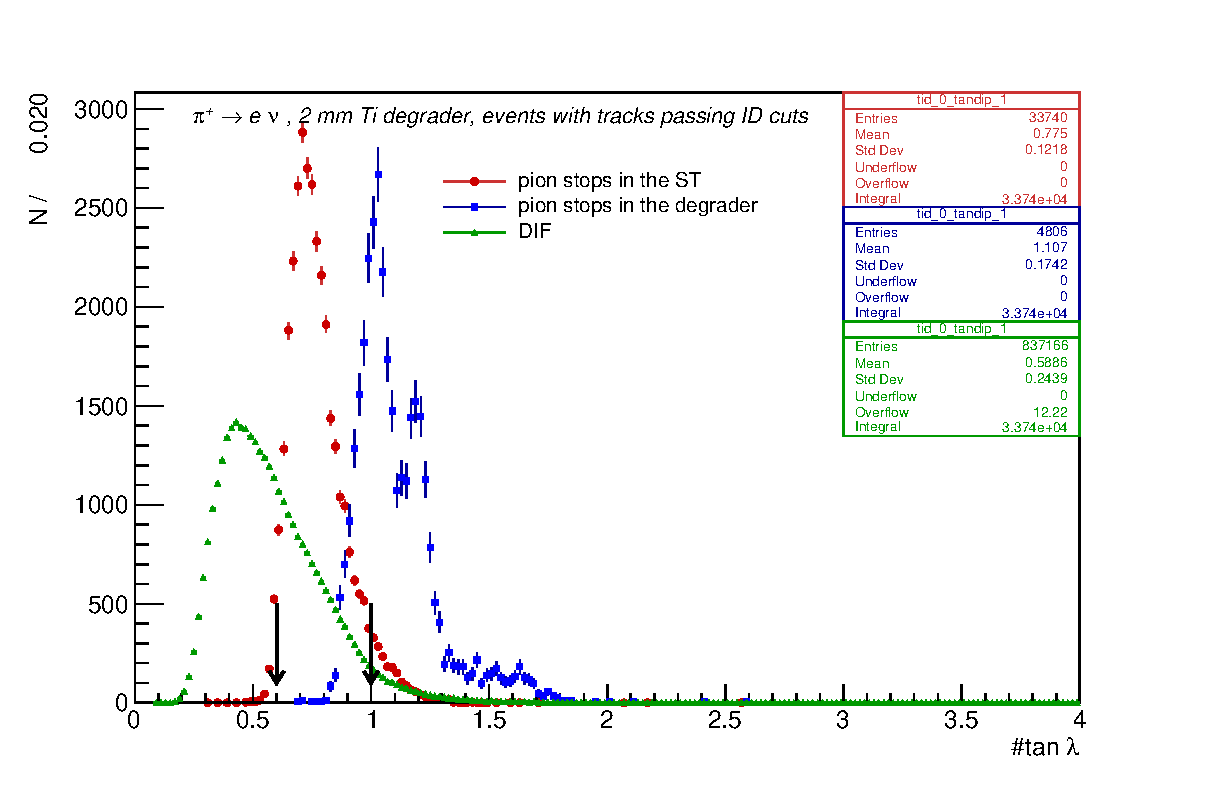
\includegraphics[width=0.55\linewidth]{pdf/figure_00273}
  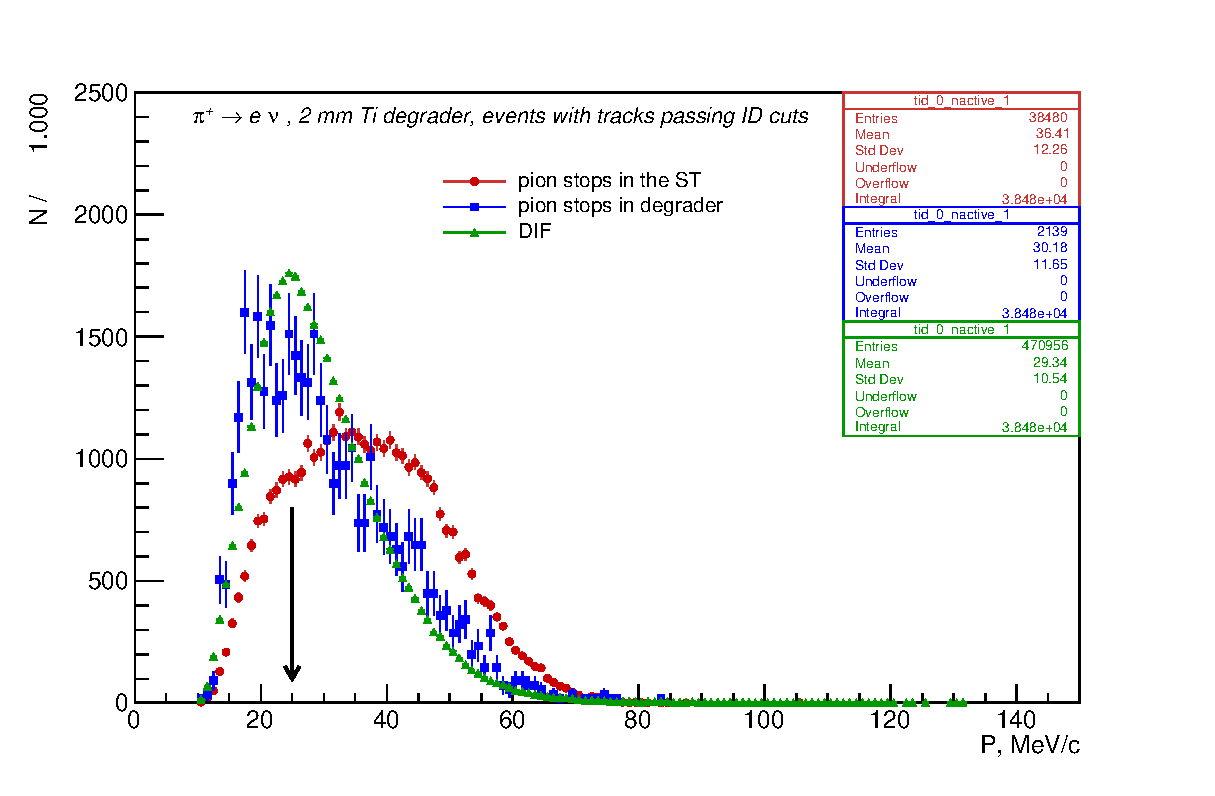
\includegraphics[width=0.55\linewidth]{pdf/figure_00274}
  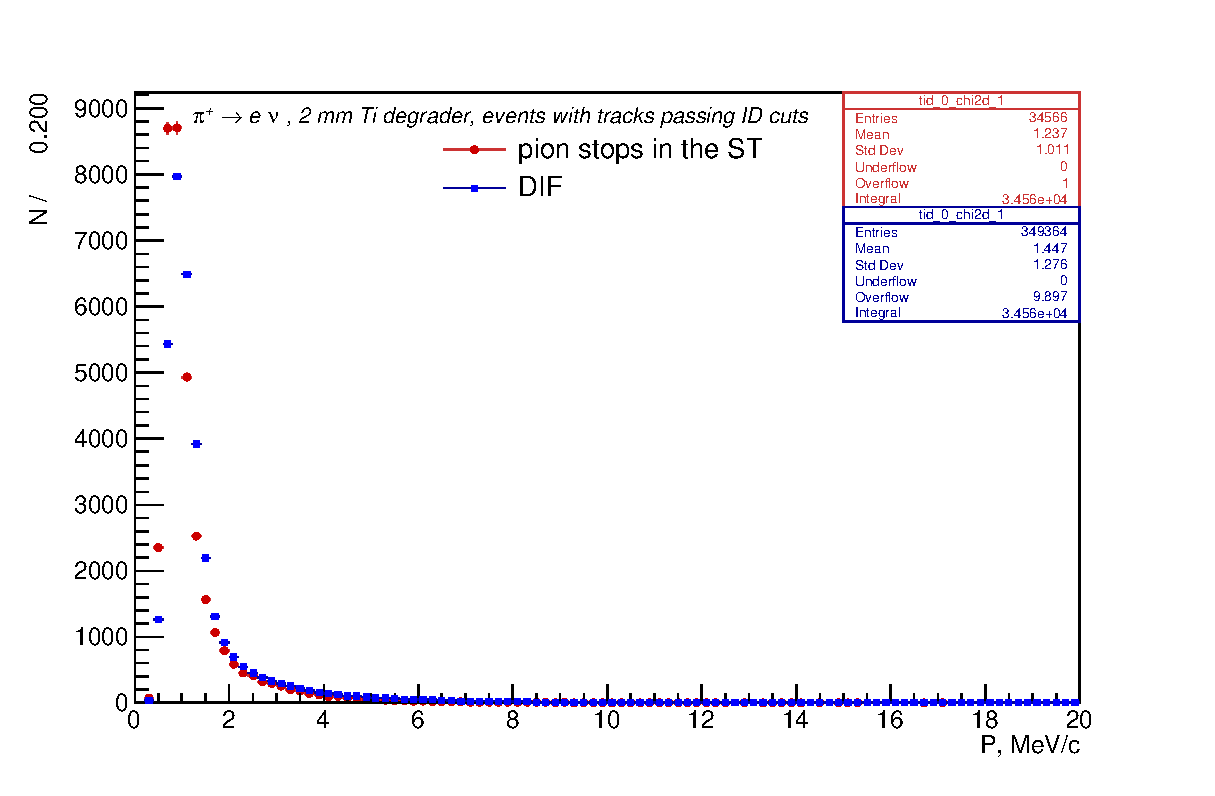
\includegraphics[width=0.55\linewidth]{pdf/figure_00275}
  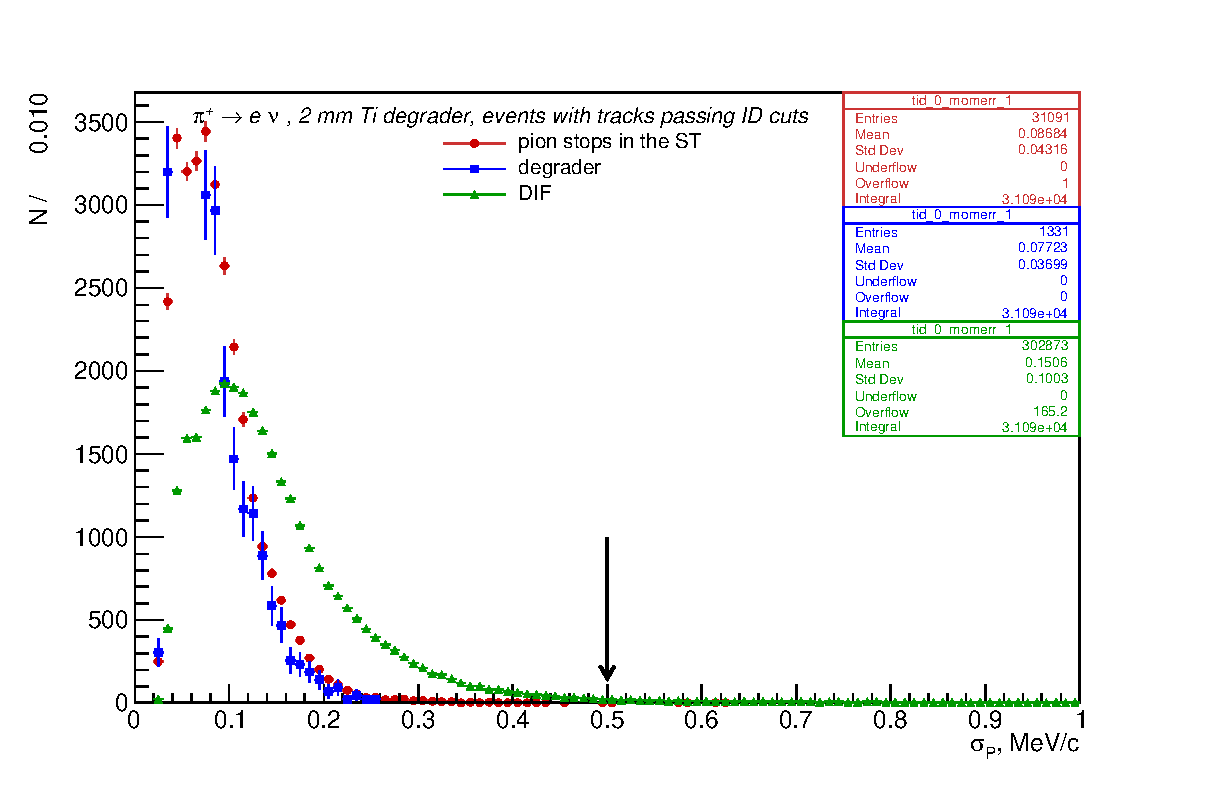
\includegraphics[width=0.55\linewidth]{pdf/figure_00276}
  \caption{
    % \label{fig:deg_vs_no_degrader_time}
    distributions of ID variables after ``N-1'' cuts
  }
\end{figure}


%%%%%%%%%%%%%%%%%%%%%%%%%%%%%%%%%%%%%%%%%%%%%%%%%%%%%%%%%%%%%%%%%%%%%%%%%%%%%%
\subsection {Signal Yields for different degrader thicknesses}
\begin{figure}[H]
  % \centering
  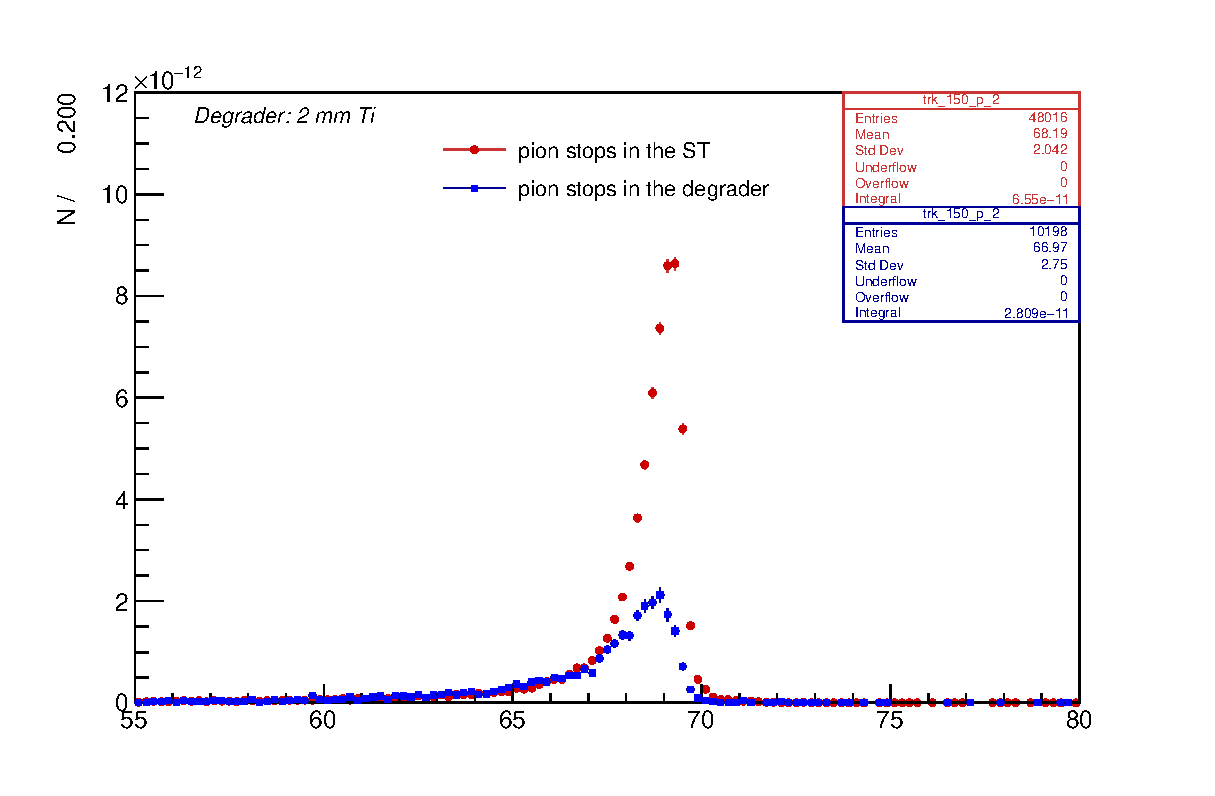
\includegraphics[width=0.55\linewidth]{pdf/figure_00251}
  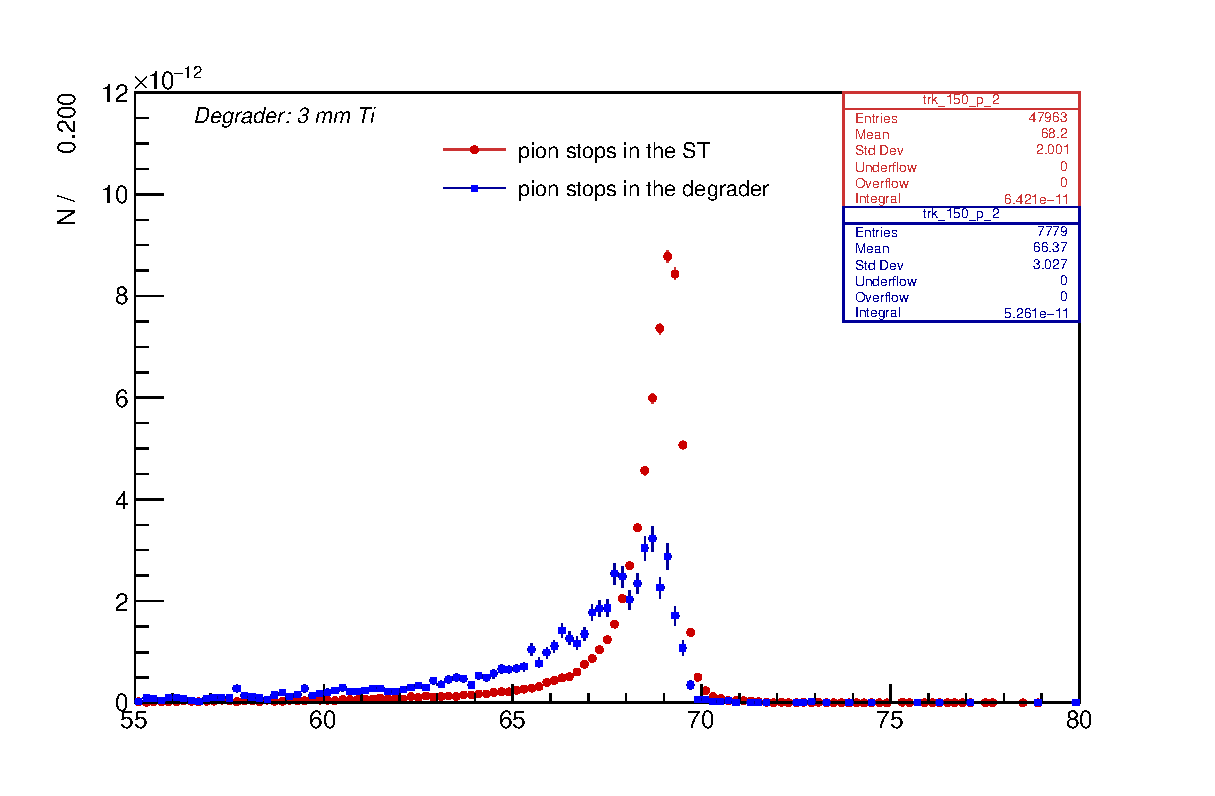
\includegraphics[width=0.55\linewidth]{pdf/figure_00351}
  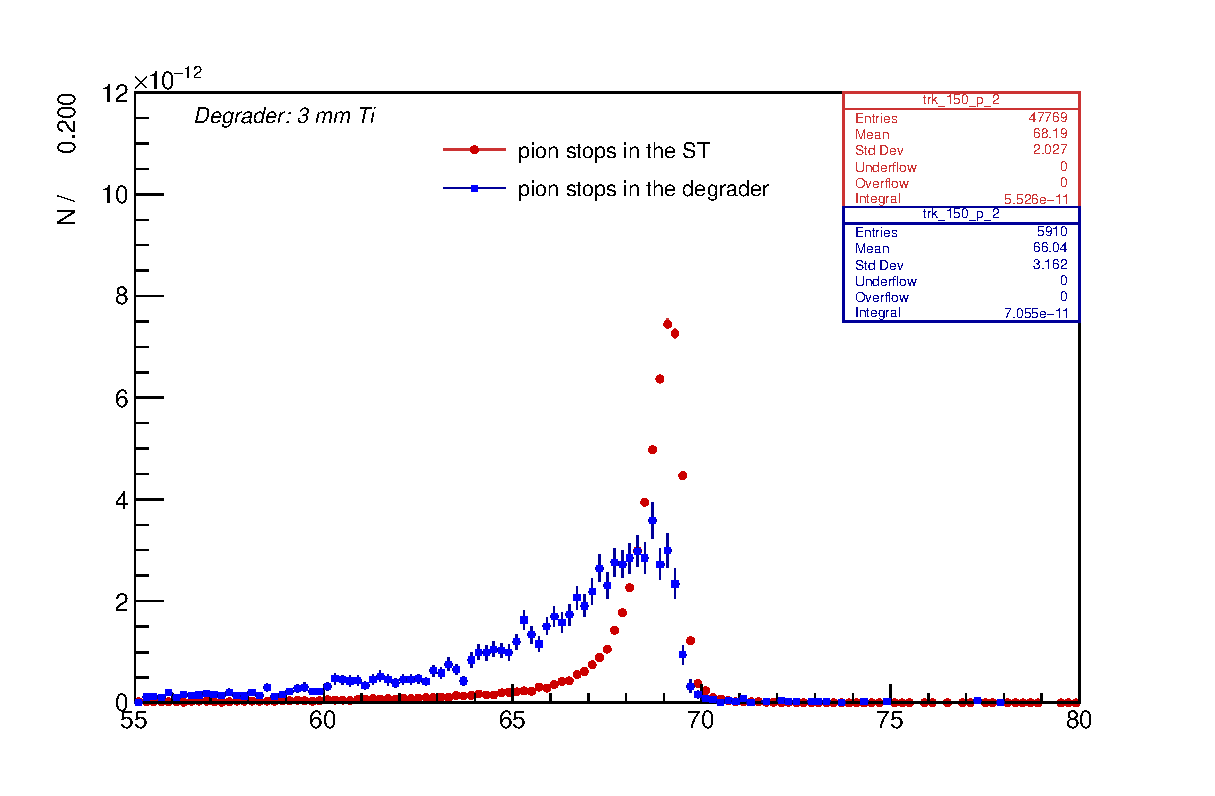
\includegraphics[width=0.55\linewidth]{pdf/figure_00451}
  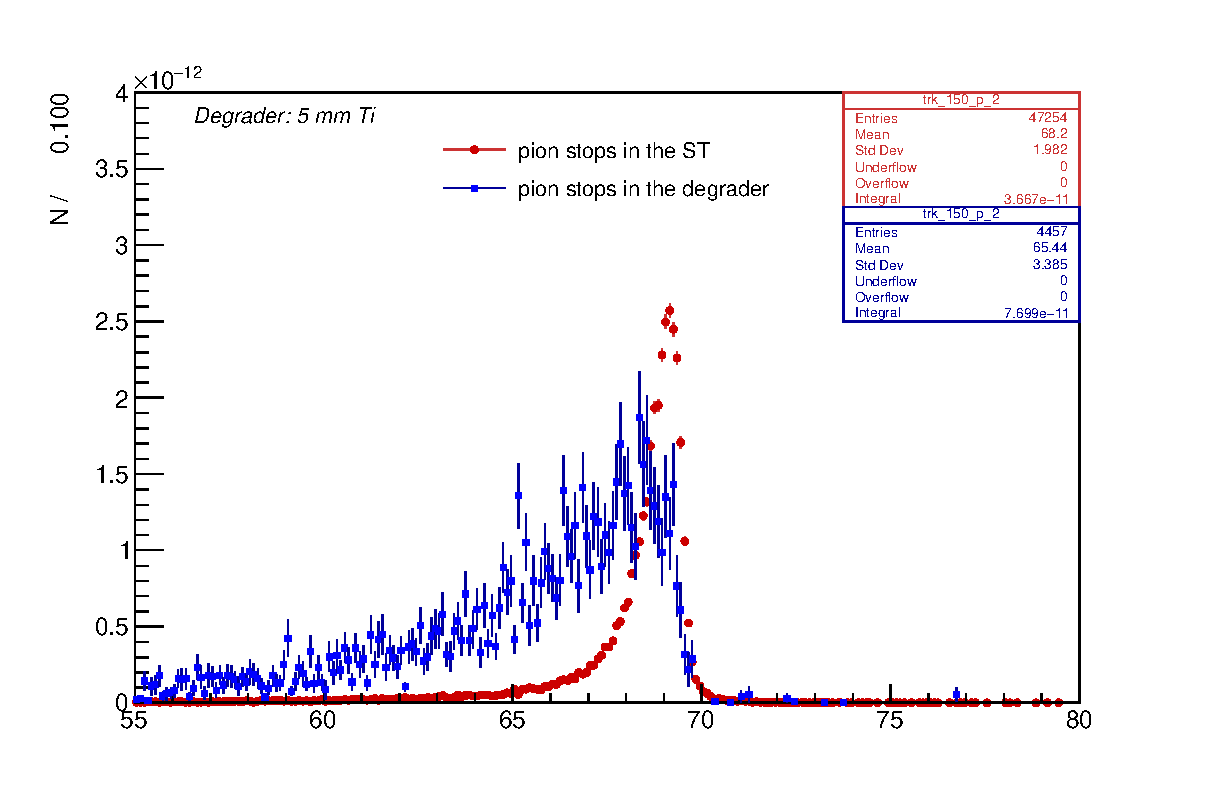
\includegraphics[width=0.55\linewidth]{pdf/figure_00551}
  \caption{
    % \label{fig:deg_vs_no_degrader_time}
  }
\end{figure}

{\red need the same plots after the track selection cuts}

%%%%%%%%%%%%%%%%%%%%%%%%%%%%%%%%%%%%%%%%%%%%%%%%%%%%%%%%%%%%%%%%%%%%%%%%%%%%%%
\subsection{Initial selection - results}




%%%%%%%%%%%%%%%%%%%%%%%%%%%%%%%%%%%%%%%%%%%%%%%%%%%%%%%%%%%%%%%%%%%%%%%%%%%%%%
\subsection{Removing muon decays in the tracker}

One of the most dangerous topologies comes from the muon decays in flight backwards in the tracker,
so a positron is produced upstream with small pZ.

In case the pattern recognition uses hits in every second station, the positrons can be misreconstructed
as particles with higher momentum.

In this case the number of hits in the time cluster is expected to be significantly higher
than the number of hits reconstructed on the track.

%%%%%%%%%%%%%%%%%%%%%%%%%%%%%%%%%%%%%%%%%%%%%%%%%%%%%%%%%%%%%%%%%%%%%%%%%%%%%%
\subsection{Tight selection - results}


\begin{figure}[H]
  % \centering
  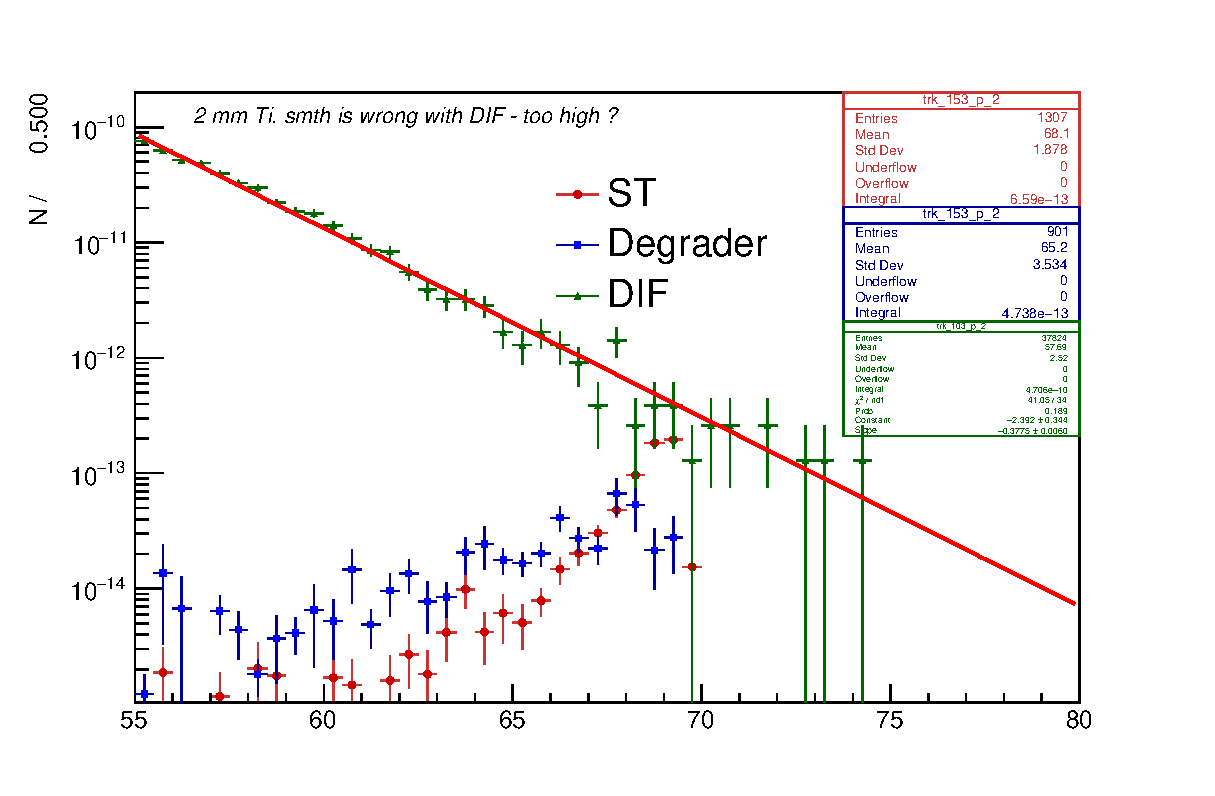
\includegraphics[width=0.55\linewidth]{pdf/figure_00231}
  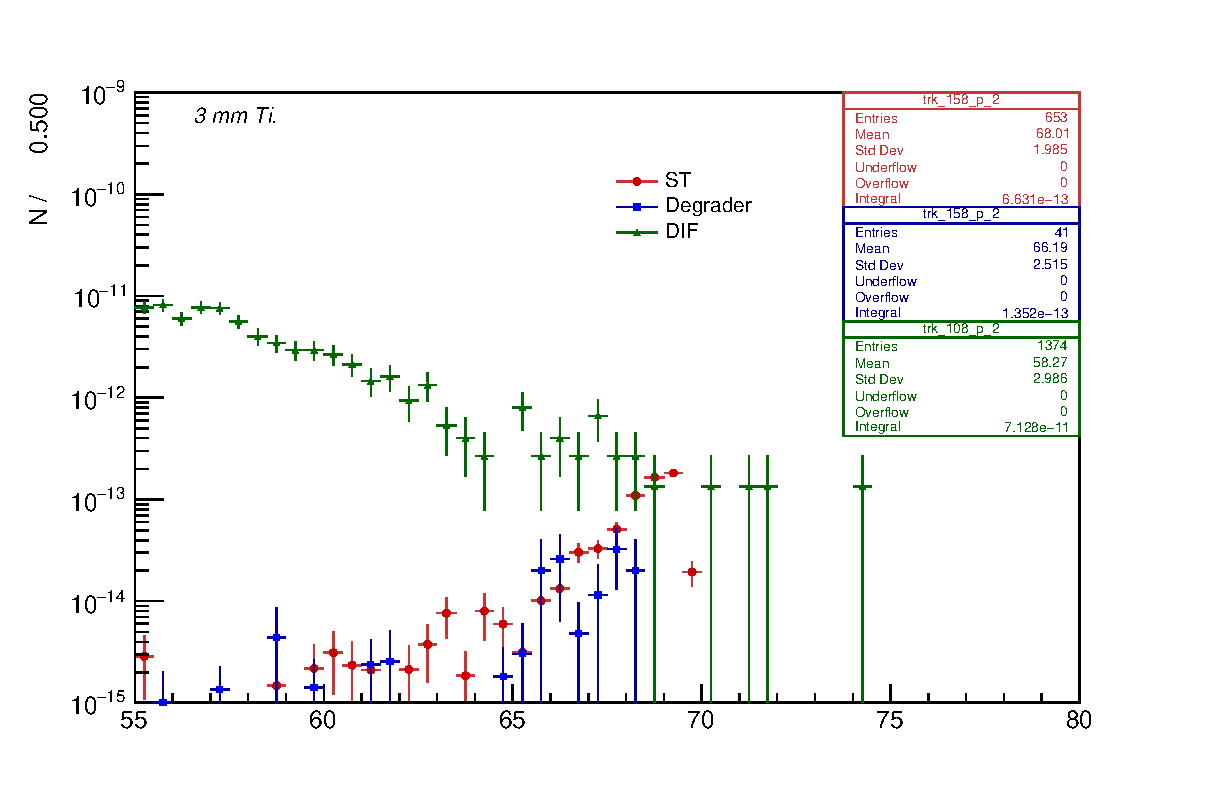
\includegraphics[width=0.55\linewidth]{pdf/figure_00331}
  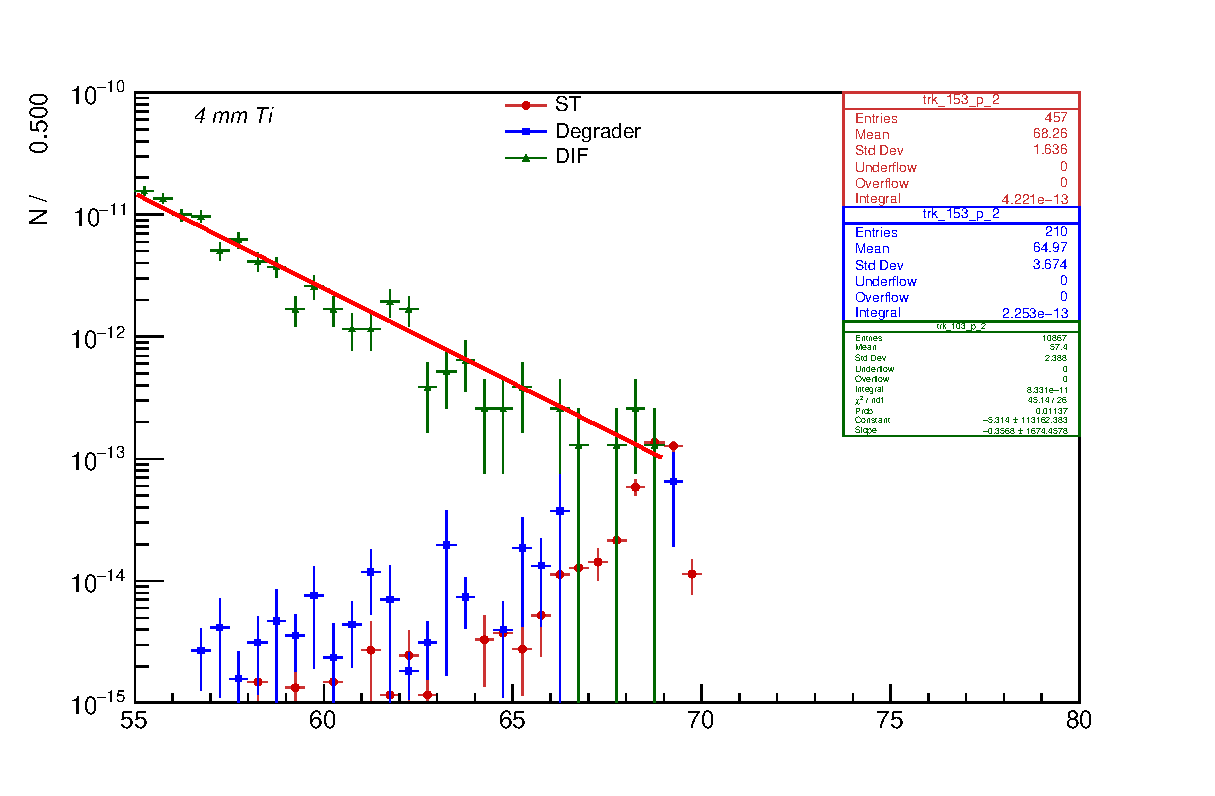
\includegraphics[width=0.55\linewidth]{pdf/figure_00431}
  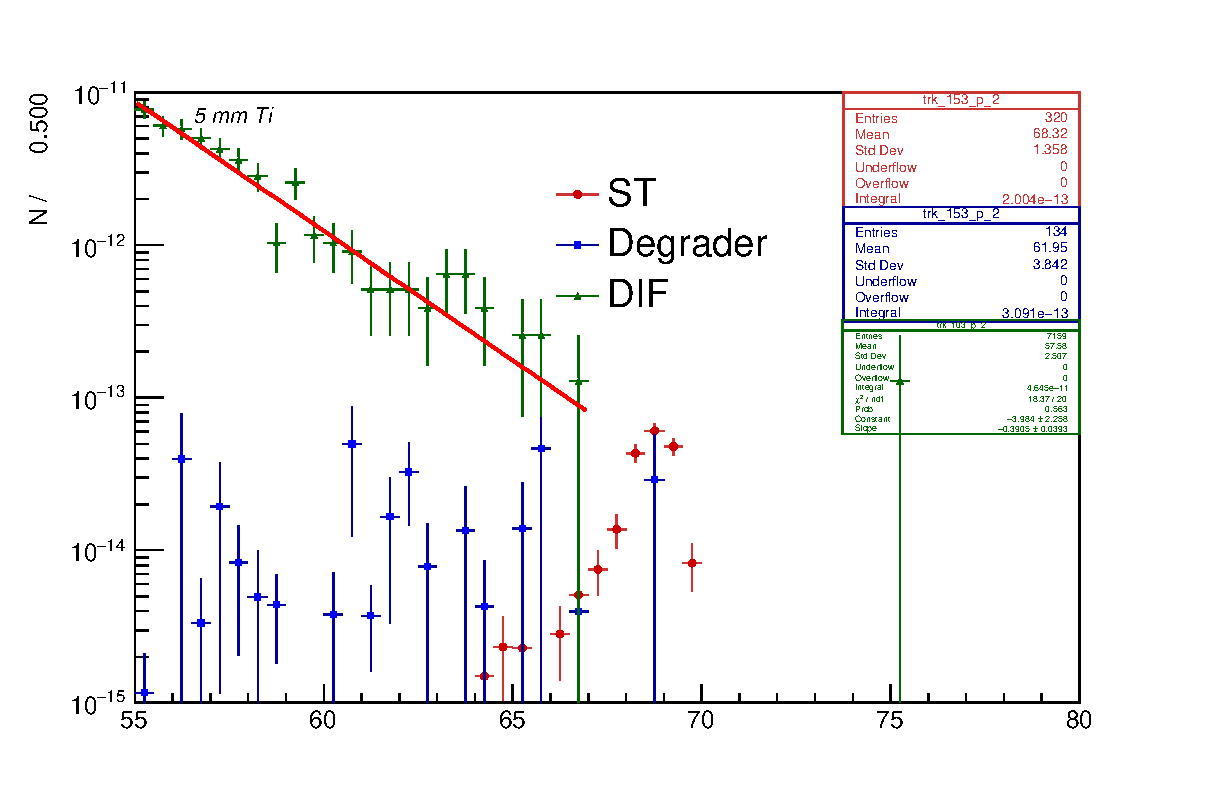
\includegraphics[width=0.55\linewidth]{pdf/figure_00531}
  \caption{
    \label{fig:deg_3mm_mom}
  }
\end{figure}

For degrader thickness of 4mm, a visual scan of DIF events above 65 MeV/c surviving
the tight selection cuts has been performed.

All surviving events represent an irreducible background and can't be rejected.

%%% Local Variables:
%%% mode: latex
%%% TeX-master: "mu2e-xxxxx"
%%% End:
